\documentclass{BHCexam}	
\renewcommand{\kongbai}{\vspace{15em}}

\newcommand{\kj}[1]{\mbox{\hspace{1pt}}\hfill\begin{tikzpicture}#1\end{tikzpicture}}
\begin{document}
\biaoti{立体几何}
\fubiaoti{}
\maketitle
\begin{questions}
\qs 在空间直角坐标系$O-xyz$中,已知$A(2,0,0),B(2,2,0),C(0,2,0),D(1,1,\sqrt{2})$,若$S_1,S_2,S_3$分别表示三棱锥$D-ABC$在$xOy,yOz,zOx$坐标平面上的正投影图形的面积,则\xx
\twoch{$S_1=S_2=S_3$}{$ S_1=S_2\text{且}S_3\ne S_1 $}{$ S_1=S_3\text{且}S_3\ne S_2 $}{$ S_2=S_3\text{且}S_1\ne S_3 $}
\qs 如图,在棱长为$2$的正方体$ ABCD-A_1B_1C_1D_1 $中,$ E $为$ BC $中点,点$ P $在线段$ D_1E $上,点$ P $到直线$ CC_1 $的距离的最小值为\tk.
\\\mbox{\hspace{1em}}\hfill
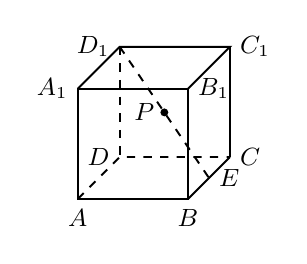
\begin{tikzpicture}[line width=0.7 pt,scale=0.7]
%\draw[help lines] (0,0) grid (3,3);
\draw (0,0) node[below](A) {\small$A$}--(2,0) node[below](B){\small$B$}--(2,2) node[right](B1){\small$B_1$}--(0,2) node[left](A1) {\small$A_1$}--(0,0)--cycle;
\draw[dashed] (0,0)--(0.76,0.76) node[left](D){\small$D$}--(2.76,0.76) node[right](C){\small$C$};
\draw (2.76,0.76)--(2,0);
\draw (0,2) --(0.76,2.76)node[left](D1){\small$D_1$}--(2.76,2.76)node[right](C1){\small$C_1$}--(2,2);
\draw [dashed](0.76,2.76)--(0.76,0.76) ;
\draw (2.76,2.76)--(2.76,0.76);
\draw [dashed](0.76,2.76)--(2.38,0.38) node[right](E) {\small$E$};
\coordinate[label=left:\small$P$] (P) at (1.57,1.57);
\draw[fill] (P) circle (1.5pt) ;
\end{tikzpicture}
\qs 如图,正方体$ ABCD-A_1B_1C_1D_1 $的棱长为$2$,动点$ E,F $在棱$ A_1B_1 $上,动点$ P,~Q $分别在棱$ AD,~CD $上,若$ EF=1,~A_1E=x,~DQ=y,~DP=z~(x,y,z\text{大于零} )$,则四面体$P-EFQ  $的体积\\
\mbox{\hspace{1pt}}\hfill\xx
\fourch{与$ x,y,z $都有关}{与$ x $有关,与$ y,z $无关}{与$ y $有关,与$ x,z $无关}{与$ z $有关,与$ x,y $无关}
\vspace{-8em}
\\\mbox{\hspace{1pt}}\hfill
\begin{tikzpicture}
\draw (0,0) node[below](A) {\small$A$}--(2,0) node[below](B){\small$B$}--(2,2) node[right](B1){\small$B_1$}--(0,2) node[left](A1) {\small$A_1$}--(0,0)--cycle;
\draw[dashed] (0,0)--(0.76,0.76) node[left](D){\small$D$}--(2.76,0.76) node[right](C){\small$C$};
\draw (2.76,0.76)--(2,0);
\draw (0,2) --(0.76,2.76)node[left](D1){\small$D_1$}--(2.76,2.76)node[right](C1){\small$C_1$}--(2,2);
\draw [dashed](0.76,2.76)--(0.76,0.76) ;
\draw (2.76,2.76)--(2.76,0.76);
%\draw [dashed](0.76,2.76)--(2.38,0.38) node[right](E) {\small$E$};
\coordinate [label=\small$E$](E) at($(A1)!0.33!(B1)$) ;
\coordinate [label=\small$F$](F) at($(A1)!0.7!(B1)$) ;
\coordinate [label=\small$P$](P) at($(0,0)!0.33!(0.76,0.76)$) ;
\coordinate [label=\small$Q$](Q) at($(D)!0.5!(C)$) ;
%\draw[fill] (E) circle (1.1pt);
%\draw[fill] (F) circle (1.1pt);
%\draw[fill] (P) circle (1.1pt);
%\draw[fill] (Q) circle (1.1pt);
\foreach \p in{E,F,P,Q}
\draw[fill](\p) circle(1.1pt);
\end{tikzpicture}
\question 
如果,在四棱锥$ P-ABCD $中,$ \text{平面}PAD\bot \text{平面}ABCD \text{,} PA\bot PD \text{,} PA=PD \text{,} AB\bot AD \text{,} AB=1\text{,}AD=2\text{,}AC=CD=\sqrt{5} $.
\begin{parts}
\part 求证:$ PD\bot \text{平面}PAB $;
\part 求直线$ PB $与平面$ PCD $所成角的正弦值;
\part 在棱$ PA $上是否存在点M,使得$ BM\sslash\text{平面 }PCD $~?若存在,求$ \dfrac{AM}{AP} $的值,若不存在,说明理由.
\end{parts}

\kj{[line cap=round,line join=round,>=triangle 45,x=0.4cm,y=0.4cm,line width=0.5pt]\clip(-5.,-2.) rectangle (5.,7.);
\draw (-4.,2.)-- (0.,6.);
\draw (0.,6.)-- (4.,2.);
\draw (4.,2.)-- (-4.,2.);
\draw (-4.,2.)-- (-2,-1.3);
\draw (-2,-1.3)-- (3.2,0.5);
\draw (3.2,0.5)-- (4.,2.);
\draw (0.,6.)-- (-2,-1.3);
\draw (0.,6.)-- (3.2,0.5);
\draw [dash pattern=on 2pt off 2pt] (-1.9752611270863778,-1.2800145850563516)-- (4.,2.);
\draw[color=black] (-4.2,2.2) node {$ D$};
\draw[color=black] (4.3,2.1) node {$ A$};
\draw[color=black] (0.2,6.2) node {$ P$};
\draw[color=black] (-2.1,-1.7) node {$ C$};
\draw[color=black] (3.6,0.4) node {$ B$};
}
\newpage

\qs
(2016·全国Ⅲ,19)如图,四棱锥$P-ABCD$中,$PA\bot\text{底面}ABCD$,$AD\sslash BC$,$AB=AD=AC=3$,$PA=BC=4$,$M$为线段$AD$上一点,$AM=2MD$,$N$为$PC$的中点.
\begin{parts}
\part 证明:$MN\sslash \text{平面}PAB$;
\part 求直线$AN$与平面$PMN$所成角的正弦值.
\end{parts}
\ct{2016III.png}
\kongbai
\qs
(2013新课标\uppercase\expandafter{\romannumeral1})如图三棱柱$ABC-A_1B_1C_1$中,侧面$BB_1C_1C$为菱形,$AB\bot B_1C$.
\begin{parts}
\part 证明$ AC=AB_1 $;
\part 若$AC\bot AB_1$,$ \angle CBB_1=60^{\circ} $,$ AB=BC $,求二面角$ A-A_1B_1-C_1 $的余弦值
\end{parts}
\kj{[line cap=round,line join=round,>=triangle 45,x=1.0cm,y=1.0cm]
\clip(-2.5,-3.5) rectangle (3.5,0.5);
\draw (0.,0.)-- (3.,0.);
\draw (-0.5,-1.5)-- (2.5,-1.5);
\draw (-2.,-3.)-- (1.,-3.);
\draw (0.,0.)-- (-2.,-3.);
\draw [dash pattern=on 1pt off 1pt] (-2.,-3.)-- (-0.5,-1.5);
\draw [dash pattern=on 1pt off 1pt] (-0.5,-1.5)-- (0.,0.);
\draw (3.,0.)-- (2.5,-1.5);
\draw (2.5,-1.5)-- (1.,-3.);
\draw (1.,-3.)-- (3.,0.);
\draw [dash pattern=on 1pt off 1pt] (-0.5,-1.5)-- (1.,-3.);
\draw [dash pattern=on 1pt off 1pt] (-2.,-3.)-- (2.5,-1.5);
\draw (0.,0.)-- (1.,-3.);
\draw [dash pattern=on 1pt off 1pt] (0.,0.)-- (0.25,-2.25);
%\begin{scriptsize}
%\draw [fill=black] (0.,0.) circle (0.5pt);
\draw[color=black] (0.09832678637091746,0.207184986069548) node {$A$};
%\draw [fill=black] (3.,0.) circle (0.5pt);
\draw[color=black] (3.1,0.2) node {$A_1$};
%\draw [fill=black] (-0.5,-1.5) circle (0.5pt);
\draw[color=black] (-0.7,-1.3547954342618216) node {$C$};
%\draw [fill=black] (2.5,-1.5) circle (0.5pt);
\draw[color=black] (2.8,-1.4036073223971768) node {$C_1$};
%\draw [fill=black] (-2.,-3.) circle (0.5pt);
\draw[color=black] (-2.216751336620222,-2.9028296008402323) node {$B$};
%\draw [fill=black] (1.,-3.) circle (0.5pt);
\draw[color=black] (1.,-3.2) node {$B_1$};}
\newpage
\qs
如图,三棱柱$ ABC-A_1B_1C_1$中,$CA=CB$,$AB=AA_1$,$\angle BAA_1=60^{\circ}$.
\begin{parts}
\part 证明 $AB\bot A_1C$;
\part $\text{若平面}ABC\bot \text{平面}AA_1B_1B$,$AB=CB=2$,求直线 $A_1C$与平面$BB_1C_1C$所成角的正弦值.
\end{parts}
\kj{[line cap=round,line join=round,>=triangle 45,x=1.2cm,y=1.2cm]
\clip(-1.,-2.5) rectangle (5.,0.8);
\draw (0.,0.)-- (4.,0.);
\draw (-0.5,-2.)-- (3.5,-2.);
\draw [dash pattern=on 1pt off 1pt] (0.5,-0.9)-- (4.5,-0.9);
\draw (0.,0.)-- (-0.5,-2.);
\draw (4.,0.)-- (3.5,-2.);
\draw (3.5,-2.)-- (4.5,-0.9);
\draw (4.5,-0.9)-- (4.,0.);
\draw [dash pattern=on 1pt off 1pt] (0.5,-0.9)-- (0.,0.);
\draw [dash pattern=on 1pt off 1pt] (0.5,-0.9)-- (-0.5,-2.);
\draw (0.,0.)-- (3.5,-2.);
\draw[color=black] (-0.15,0.05) node {$C$};
\draw[color=black] (4.2,0.1) node {$C_1$};
\draw[color=black] (-0.7,-1.9) node {$A$};
\draw[color=black] (3.5,-2.2) node {$A_1$};
\draw[color=black] (0.55,-1.1) node {$B$};
\draw[color=black] (4.7,-1) node {$B_1$}; 
}
\kongbai
\qs (2012理)如图$1$,在$Rt\triangle ABC$中,$\angle C=90^{\circ}$,$ BC=3,~AC=6,~D,~E $分别是$ AC,~AB $上的点,且$ DE\sslash BC,~DE=2 $,将$ \triangle ADE $沿$ DE $折起到$ \triangle A_1DE $的位置,使$ A_1C\bot CD $,如图2.
\begin{parts}
\part 求证:$ A_1C\bot \text{平面}BCDE $;
\part 若$ M $是$ A_1D $的中点,求$ CM $与平面$ A_1BE $所成角的大小;
\part 线段$ BC $上是否存在点$ P $,使平面$ A_1DP $与平面$ A_1BE $垂直?说明理由.
\end{parts}
%\vspace{-5em}
\kj{[scale=0.6,line width=0.6pt]\coordinate[label=left:\scriptsize$C$] (C) at (0,0);
\coordinate [label=above:\scriptsize$A$](A) at (0,6);
\coordinate[label=left:\scriptsize$D$] (D) at (0,2);
\coordinate [label=right:\scriptsize$B$](B) at (3,0);
\coordinate [label=right:\scriptsize$E$](E) at (2,2);
\draw (C)--(D)--(A)--(E)--(B)--cycle;
\draw (D)--(E);

%\draw[xshift=5cm] (0,0) grid (3,3);
\draw[xshift=5cm](0,0)node[below ]{\scriptsize$C$}--(3,0)node[below]{\scriptsize$B$}--(0,4) node[above](A1){\scriptsize$A_1$}--cycle ;
\draw[xshift=5cm,dashed] (0,0)--(0.75,0.85)node[above right](D1){\scriptsize$D$}--(2.7,0.85)node[right]{\scriptsize$E$};
\draw[xshift=5cm](2.7,0.85)--(3,0);
\draw[xshift=5cm,dashed] (0,4)--(0.75,0.85);
\draw[xshift=5cm](0,4)--(2.7,0.85);
\draw[xshift=5cm,dashed](0,0)--(0.375,2.425) node[right]{\scriptsize $M$};}
\kongbai
\qs (2012文)如图$1$,在$Rt\triangle ABC$中,$\angle C=90^{\circ}$,$D,E$分别为$AC$,$AB$的中点,点$F$为线段$CD$上的一点.将$\triangle ADE$沿$DE$折起到$\triangle A_1DE$的位置,使$A_1F\bot CD$,如图$2$.
\begin{parts}
\part 求证:$DE\sslash \text{平面}A_1CB$;
\part 求证:$A_1F\bot BE$;
\part 线段$ A_1B $上是否存在点$ Q $,使得$ A_1C\bot\text{平面}DEQ $?说明理由.
\end{parts}% \vspace{-5em}
\kj{[scale=0.6,line width=0.6pt]\coordinate[label=left:\scriptsize$C$] (C) at (0,0);
\coordinate [label=above:\scriptsize$A$](A) at (0,6);
\coordinate[label=left:\scriptsize$F$] (F) at (0,1);
\coordinate[label=left:\scriptsize$D$] (D) at (0,2);
\coordinate [label=right:\scriptsize$B$](B) at (3,0);
\coordinate [label=right:\scriptsize$E$](E) at (2,2);
\draw (C)--(D)--(A)--(E)--(B)--cycle;
\draw (D)--(E);

%\draw[xshift=5cm] (0,0) grid (3,3);
\draw[xshift=5cm](0,0)node[below ]{\scriptsize$C$}--(3,0)node[below]{\scriptsize$B$}--(0,4) node[above](A1){\scriptsize$A_1$}--cycle ;
\draw[xshift=5cm,dashed] (0,0)--(0.325,0.425) node[right](F){\scriptsize $F$}--(0.75,0.85)node[above right](D1){\scriptsize$D$}--(2.7,0.85)node[right]{\scriptsize$E$};
\draw[xshift=5cm](2.7,0.85)--(3,0);
\draw[xshift=5cm,dashed] (0,4)--(0.75,0.85) (0,4)--(0.325,0.425);
\draw[xshift=5cm](0,4)--(2.7,0.85) ;}
%\draw[xshift=5cm,dashed](0,0)--(0.375,2.425) node[right]{\scriptsize $M$};
\kongbai
\qs 如图,在四棱锥$ P-ABCD $中,$ AB\sslash CD ,~AB\bot AD,~CD=2AB$,$ \text{PAD}\bot \text{底面}ABCD $,$ PA\bot AD $,$ E\text{和}F $分别是$ CD $和$ PC $的中点,求证:
\begin{parts}
\part $PA\bot \text{底面}ABCD$;
\part $ BE\sslash \text{平面}PAD $;
\part 平面$ BEF \bot \text{平面}PCD$
\end{parts}
\vspace{-6em}
\ct{2013wen.png}
\newpage
\qs 如图,在四棱锥$ P-ABCD $中,$ PA\bot \text{平面}ABCD $,底面$ ABCD $是菱形,$ AB=2,~\angle BAD=60^{\circ} $.
\begin{parts}
\part 求证:$ BD\bot \text{平面}PAC $;
\part 若$ PA=AB $,求$ PB $与$ AC $所成角的余弦值;
\part 当平面$ PBC $与平面$ PCD $垂直时,求$ PA $的长.
\end{parts}
\vspace{-5em}
\kj{[scale=0.8]\coordinate[label=left:$A$] (A) at (0,0); 
\coordinate[label=above:\small$P$](P) at (0,4);
\coordinate[label=below:\small$B$](B) at (1.5,-0.8);
\coordinate[label=above:\small$D$](D) at (2.5,0.8);
\coordinate[label=right:\small$C$](C) at (4,0);
\draw (A)--(B)--(C);
\draw[dashed](A)--(D)--(C) (P)--(D) (A)--(C) (B)--(D);
\draw(P)--(A) (P)--(B) (P)--(C);
}

\end{questions}
\end{document}
